\section{Documentos y Código}
\subsection{Documentación}
\begin{compactitem}
  \item \href{https://github.com/dexaxi/TFG_Unity_Package/blob/main/Assets/DUJAL/Documentation/DUJAL%20Documentation.pdf}{Documentación}
  \item \href{https://github.com/dexaxi/TFG_Unity_Package/blob/main/Assets/DUJAL/Documentation/Memoria%20TFG%20%C3%81ngel%20Baeza%20S%C3%A1nchez.pdf}{Memoria}
  \item \href{https://docs.google.com/forms/d/e/1FAIpQLSd1cEq_ghDKNGu-EFjOm2AS5huoM882GzUzjwZkY_DLQak9Fw/viewform?usp=sharing&ouid=100594158238727737282}{Cuestionario}
\end{compactitem}

\subsection{Repositorios}
\begin{compactitem}
  \item DUJAL: \url{https://github.com/dexaxi/TFG_unity_package}
  \item UniTask: \url{https://github.com/Cysharp/UniTask}
\end{compactitem}


\section{Tablas y figuras}
\subsection{Resultados del Cuestionario}
% Insertar una figura
\begin{figure}[H]
  \centering
  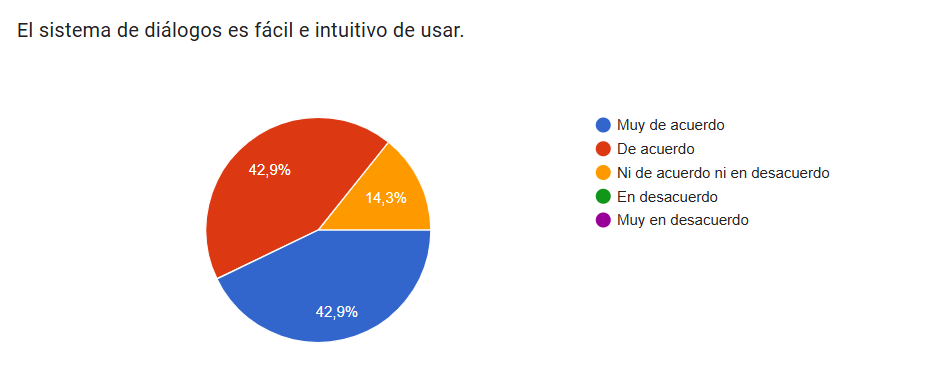
\includegraphics[width=450px,clip=true]{CUESTIONARIO_1.png}
  \caption{Encuesta sobre la facilidad de uso del sistema de diálogo.}
  \label{fig:CUESTIONARIO_1}
\end{figure}
\raggedbottom

\begin{figure}[H]
  \centering
  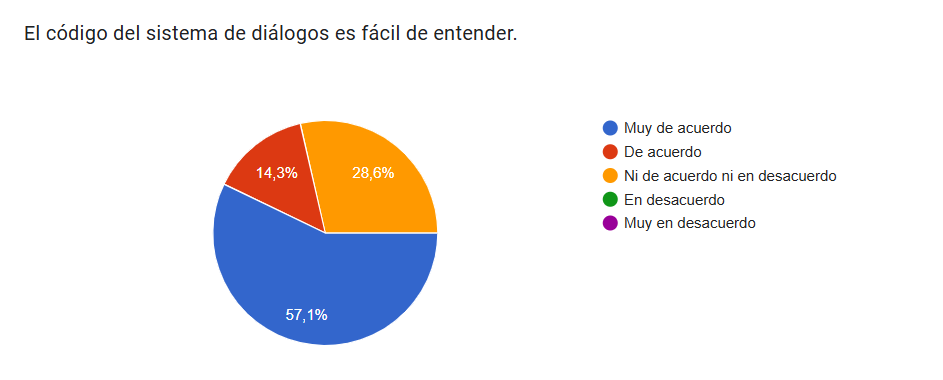
\includegraphics[width=450px,clip=true]{CUESTIONARIO_2.png}
  \caption{Encuesta sobre la calidad del código del sistema de diálogo.}
  \label{fig:CUESTIONARIO_2}
\end{figure}
\raggedbottom

\begin{figure}[H]
  \centering
  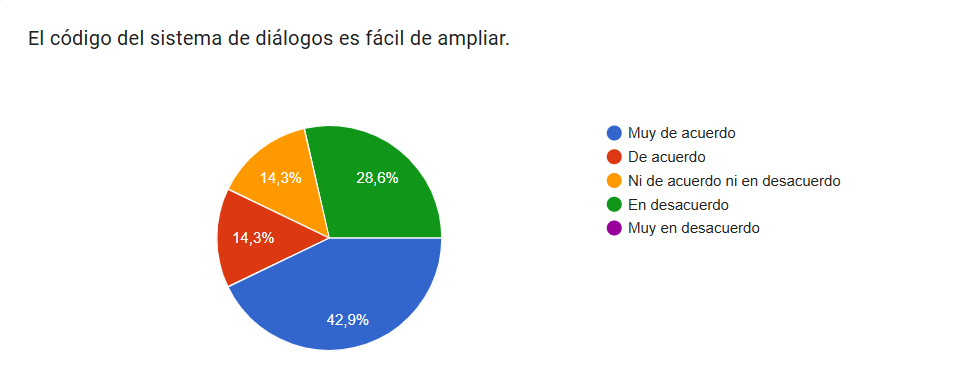
\includegraphics[width=450px,clip=true]{CUESTIONARIO_3.png}
  \caption{Encuesta sobre la escalabilidad del sistema de diálogo.}
  \label{fig:CUESTIONARIO_3}
\end{figure}
\raggedbottom

\begin{figure}[H]
  \centering
  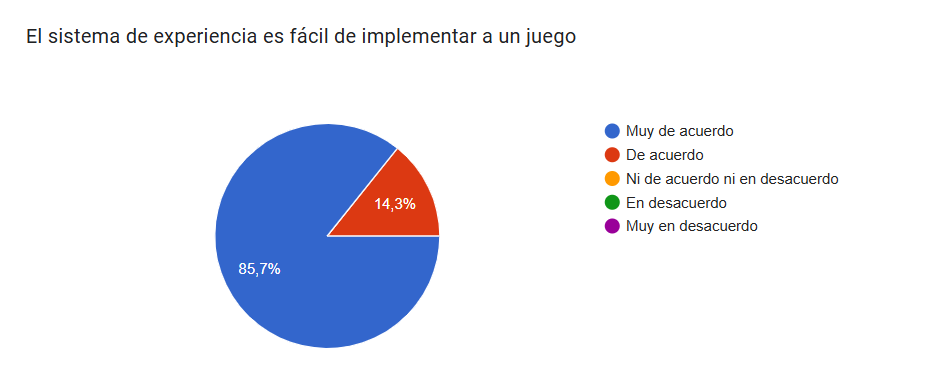
\includegraphics[width=450px,clip=true]{CUESTIONARIO_4.png}
  \caption{Encuesta sobre la facilidad de uso del sistema de experiencia.}
  \label{fig:CUESTIONARIO_4}
\end{figure}
\raggedbottom

\begin{figure}[H]
  \centering
  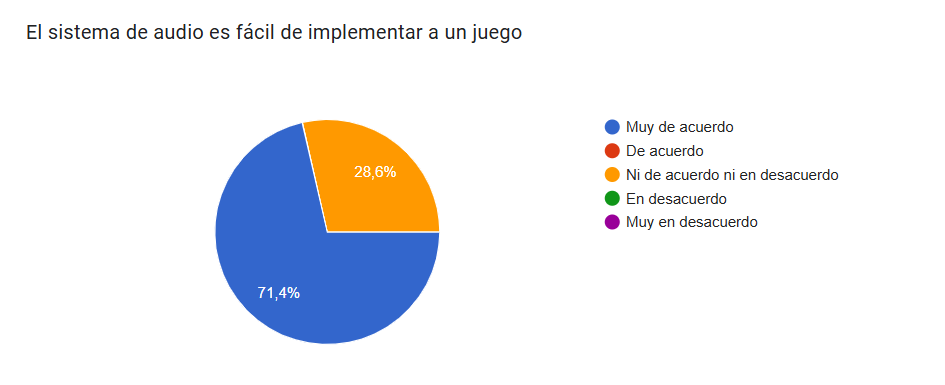
\includegraphics[width=450px,clip=true]{CUESTIONARIO_5.png}
  \caption{Encuesta sobre la facilidad de uso del sistema de audio.}
  \label{fig:CUESTIONARIO_5}
\end{figure}
\raggedbottom

\begin{figure}[H]
  \centering
  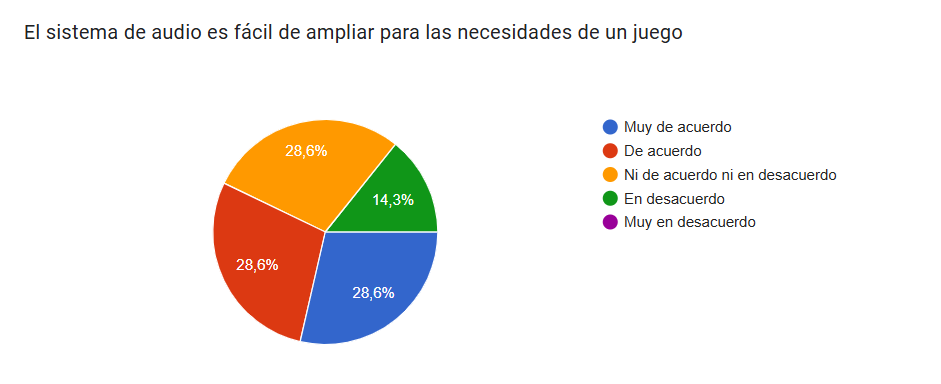
\includegraphics[width=450px,clip=true]{CUESTIONARIO_6.png}
  \caption{Encuesta sobre la escalabilidad del sistema de audio.}
  \label{fig:CUESTIONARIO_6}
\end{figure}
\raggedbottom

\begin{figure}[H]
  \centering
  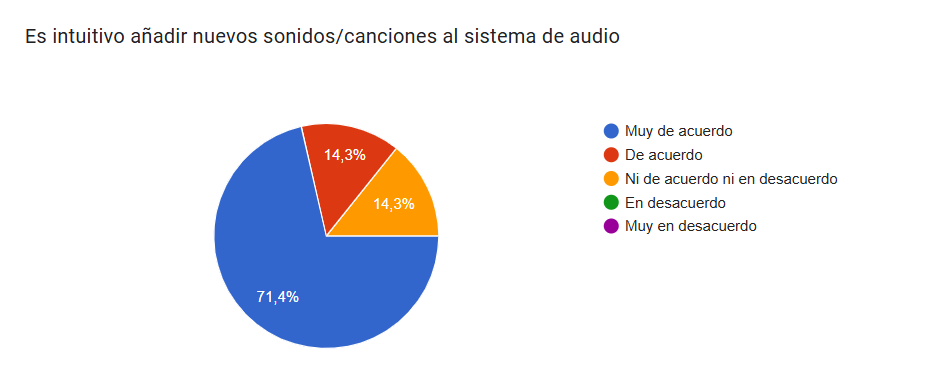
\includegraphics[width=450px,clip=true]{CUESTIONARIO_7.png}
  \caption{Encuesta sobre la adaptabilidad del sistema de audio.}
  \label{fig:CUESTIONARIO_7}
\end{figure}
\raggedbottom

\begin{figure}[H]
  \centering
  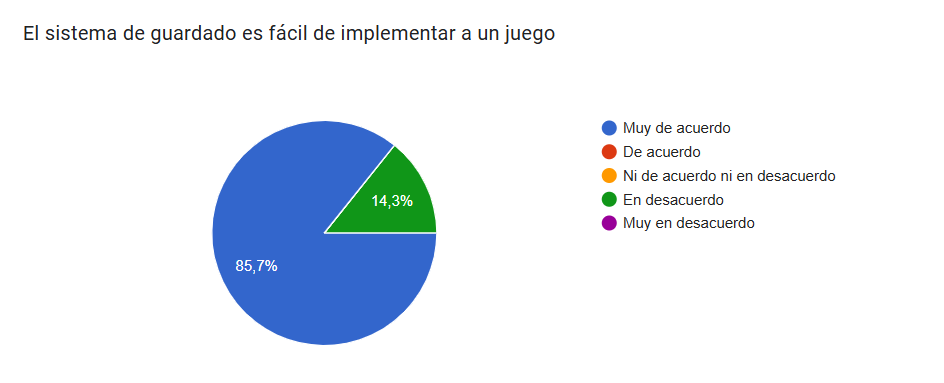
\includegraphics[width=450px,clip=true]{CUESTIONARIO_8.png}
  \caption{Encuesta sobre la facilidad de uso del sistema de guardado.}
  \label{fig:CUESTIONARIO_8}
\end{figure}
\raggedbottom

\begin{figure}[H]
  \centering
  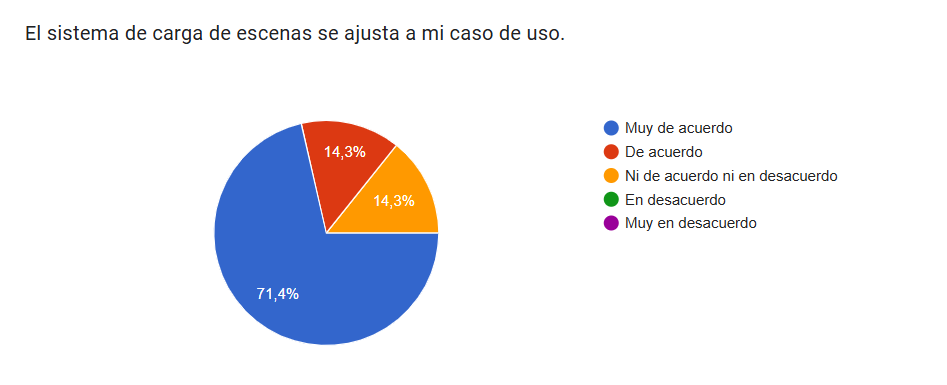
\includegraphics[width=450px,clip=true]{CUESTIONARIO_9.png}
  \caption{Encuesta sobre la utilidad del sistema de carga de escenas.}
  \label{fig:CUESTIONARIO_9}
\end{figure}
\raggedbottom

\begin{figure}[H]
  \centering
  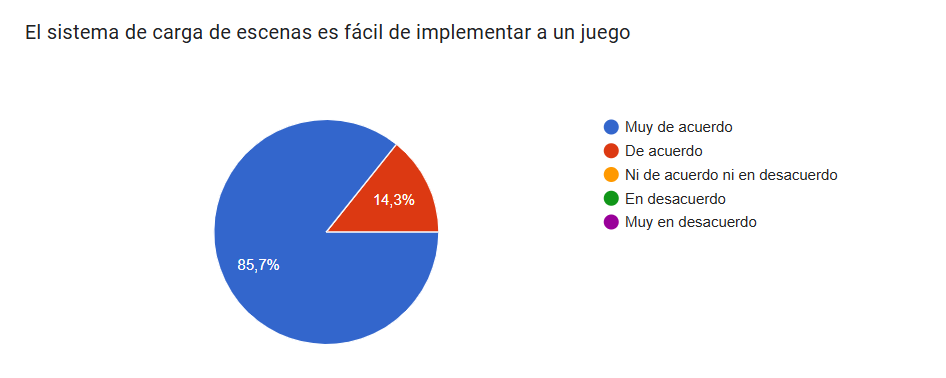
\includegraphics[width=450px,clip=true]{CUESTIONARIO_10.png}
  \caption{Encuesta sobre la facilidad de uso del sistema de carga de escenas.}
  \label{fig:CUESTIONARIO_10}
\end{figure}
\raggedbottom

\begin{figure}[H]
  \centering
  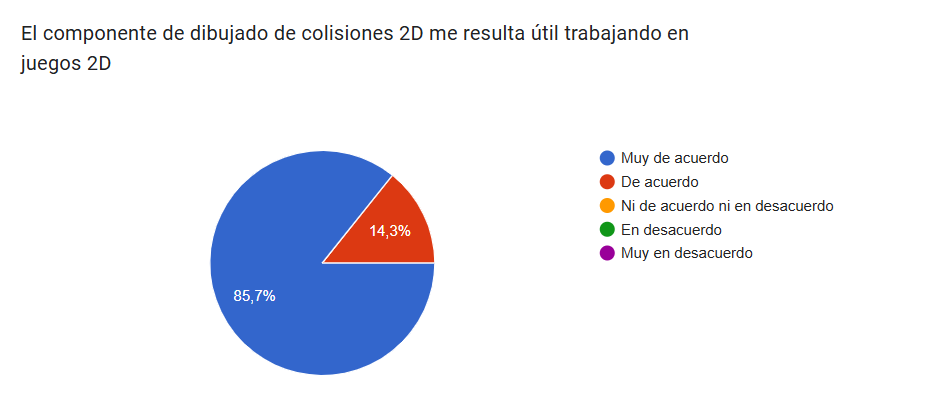
\includegraphics[width=450px,clip=true]{CUESTIONARIO_11.png}
  \caption{Encuesta sobre la utilidad del sistema de dibujado de colisiones 2D.}
  \label{fig:CUESTIONARIO_11}
\end{figure}
\raggedbottom

\begin{figure}[H]
  \centering
  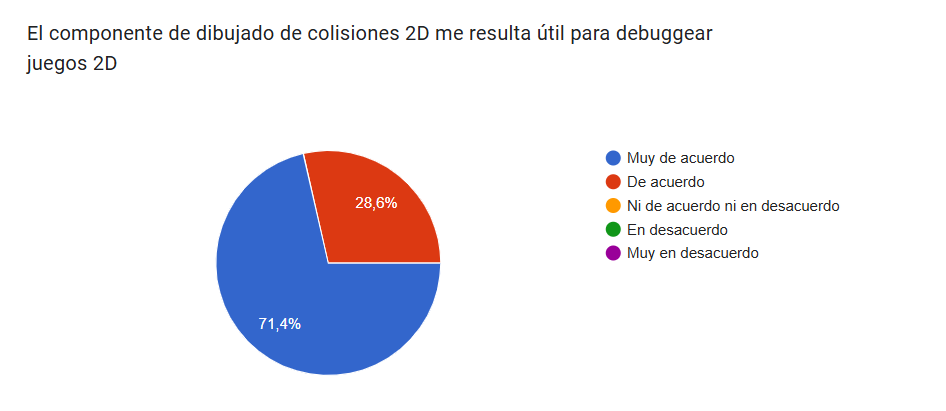
\includegraphics[width=450px,clip=true]{CUESTIONARIO_12.png}
  \caption{Encuesta sobre el cumplimiento de la funcionalidad del sistema de dibujado de colisiones 2D.}
  \label{fig:CUESTIONARIO_12}
\end{figure}
\raggedbottom

\begin{figure}[H]
  \centering
  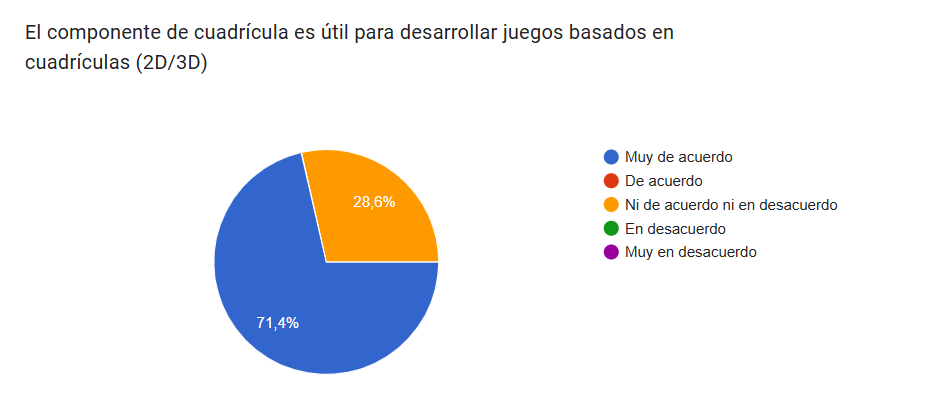
\includegraphics[width=450px,clip=true]{CUESTIONARIO_13.png}
  \caption{Encuesta sobre la utilidad del componente de cuadrícula.}
  \label{fig:CUESTIONARIO_13}
\end{figure}
\raggedbottom

\begin{figure}[H]
  \centering
  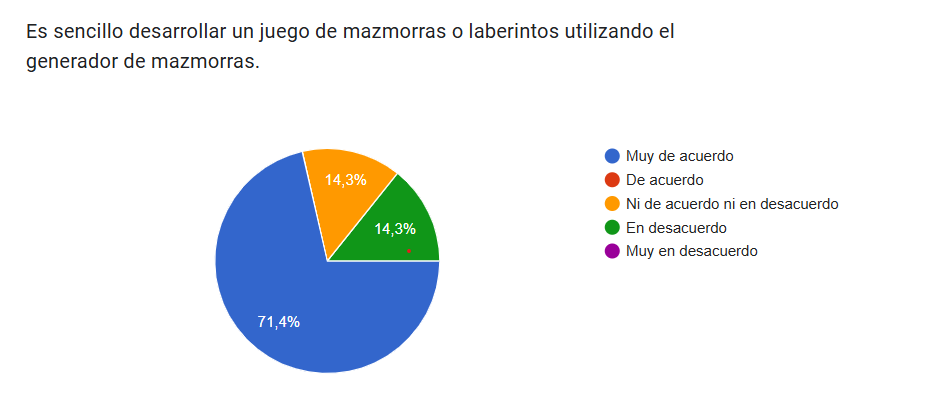
\includegraphics[width=450px,clip=true]{CUESTIONARIO_14.png}
  \caption{Encuesta sobre la facilidad de uso del sistema de mazmorras.}
  \label{fig:CUESTIONARIO_14}
\end{figure}
\raggedbottom

\begin{figure}[H]
  \centering
  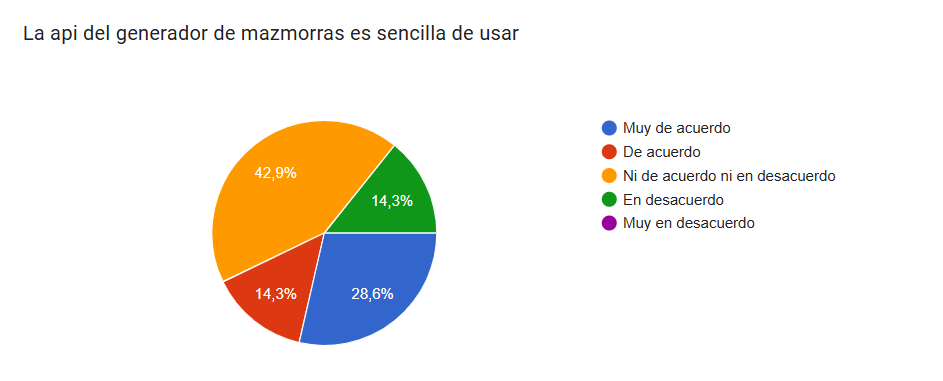
\includegraphics[width=450px,clip=true]{CUESTIONARIO_15.png}
  \caption{Encuesta sobre la sencillez del código del sistema de mazmorras.}
  \label{fig:CUESTIONARIO_15}
\end{figure}
\raggedbottom

\begin{figure}[H]
  \centering
  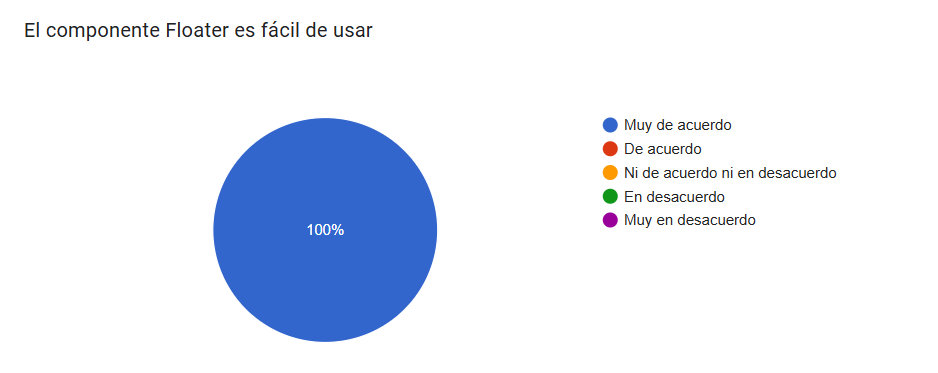
\includegraphics[width=450px,clip=true]{CUESTIONARIO_16.png}
  \caption{Encuesta sobre la facilidad de uso del componente Floater.}
  \label{fig:CUESTIONARIO_16}
\end{figure}
\raggedbottom

\begin{figure}[H]
  \centering
  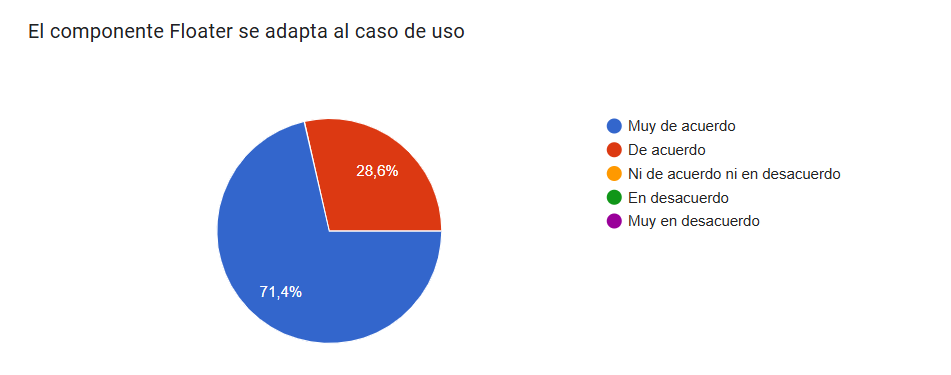
\includegraphics[width=450px,clip=true]{CUESTIONARIO_17.png}
  \caption{Encuesta sobre la utilidad del componente Floater.}
  \label{fig:CUESTIONARIO_17}
\end{figure}
\raggedbottom

\begin{figure}[H]
  \centering
  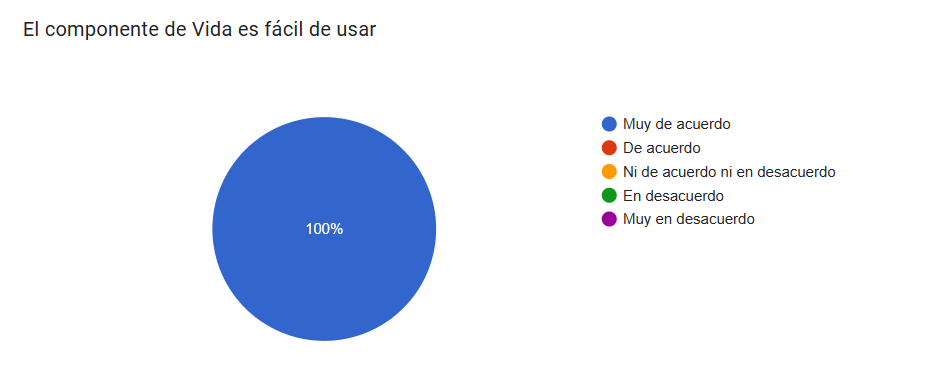
\includegraphics[width=450px,clip=true]{CUESTIONARIO_18.png}
  \caption{Encuesta sobre la facilidad de uso del componente de vida. }
  \label{fig:CUESTIONARIO_18}
\end{figure}
\raggedbottom

\begin{figure}[H]
  \centering
  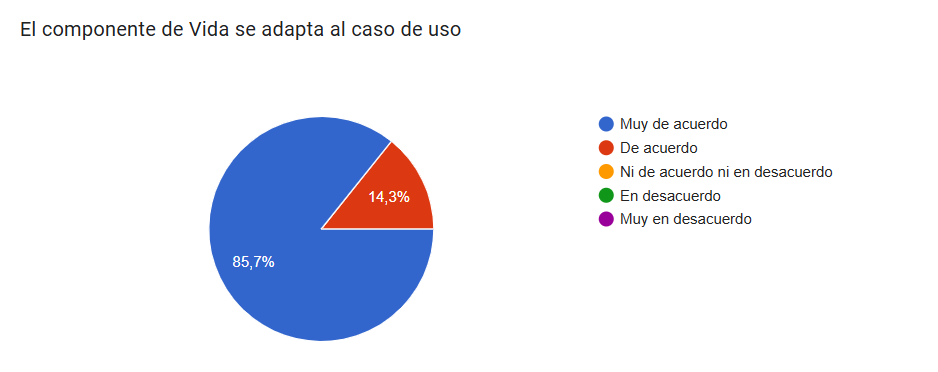
\includegraphics[width=450px,clip=true]{CUESTIONARIO_19.png}
  \caption{Encuesta sobre la utilidad del componente de vida. }
  \label{fig:CUESTIONARIO_19}
\end{figure}
\raggedbottom

\begin{figure}[H]
  \centering
  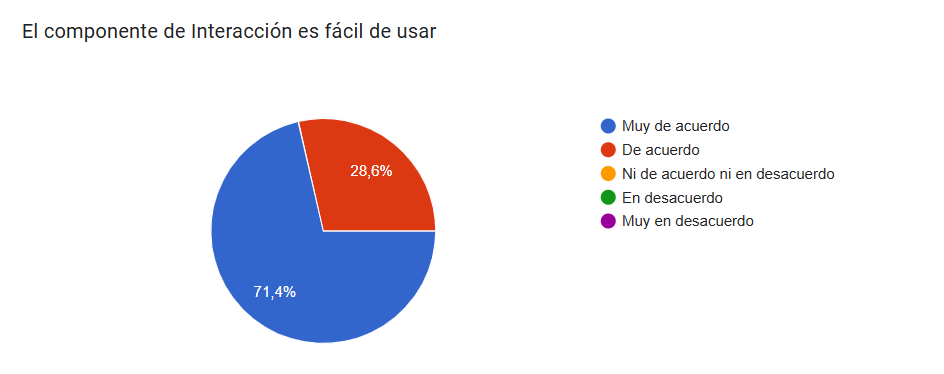
\includegraphics[width=450px,clip=true]{CUESTIONARIO_20.png}
  \caption{Encuesta sobre la facilidad de uso del componente de interacción.}
  \label{fig:CUESTIONARIO_20}
\end{figure}
\raggedbottom

\begin{figure}[H]
  \centering
  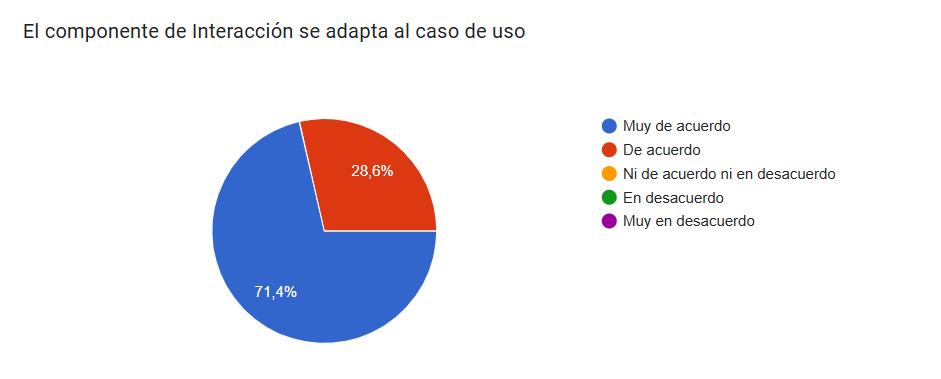
\includegraphics[width=450px,clip=true]{CUESTIONARIO_21.png}
  \caption{Encuesta sobre la utilidad del componente de interacción.}
  \label{fig:CUESTIONARIO_21}
\end{figure}
\raggedbottom

\begin{figure}[H]
  \centering
  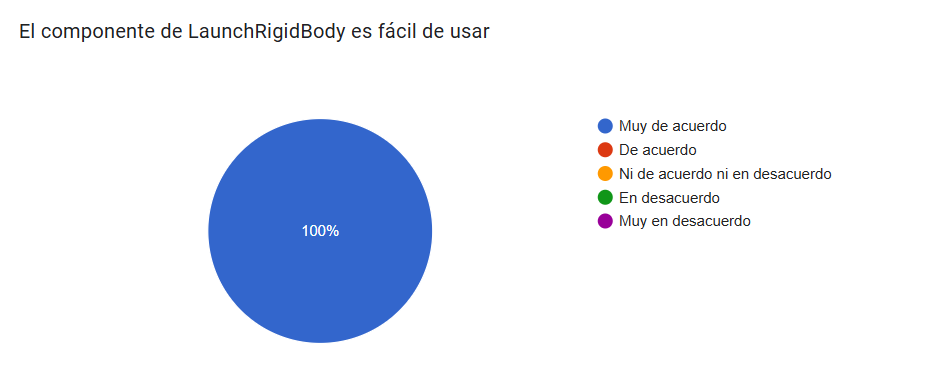
\includegraphics[width=450px,clip=true]{CUESTIONARIO_22.png}
  \caption{Encuesta sobre la facilidad de uso del componente LaunchRigidbody.}
  \label{fig:CUESTIONARIO_22}
\end{figure}
\raggedbottom

\begin{figure}[H]
  \centering
  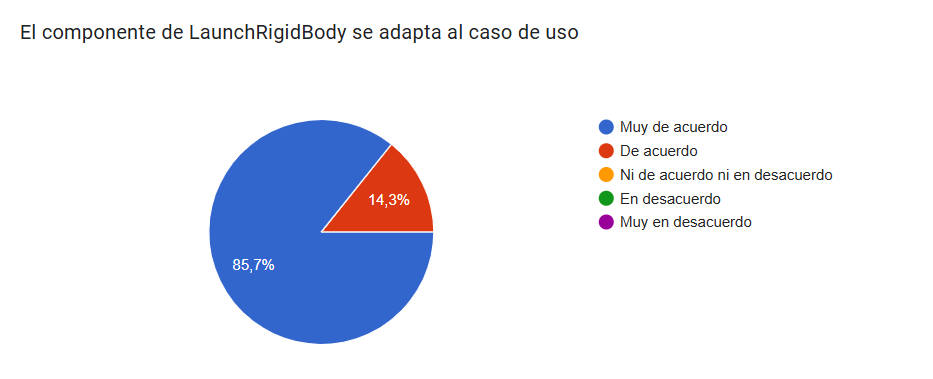
\includegraphics[width=450px,clip=true]{CUESTIONARIO_23.png}
  \caption{Encuesta sobre la utilidad del componente LaunchRigidbody.}
  \label{fig:CUESTIONARIO_23}
\end{figure}
\raggedbottom

\begin{figure}[H]
  \centering
  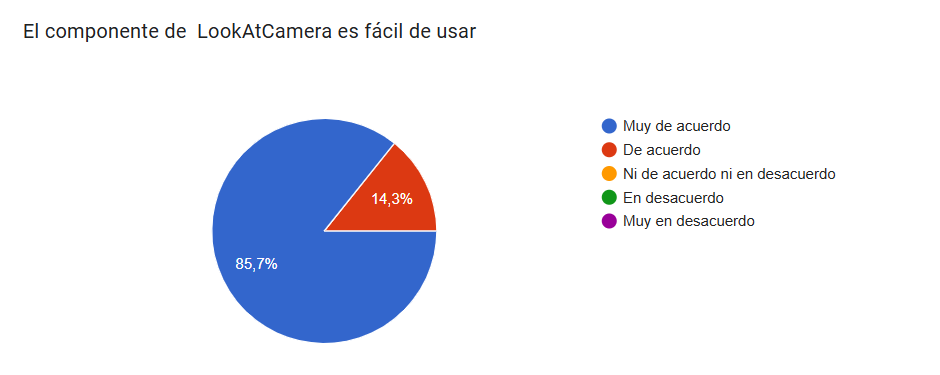
\includegraphics[width=450px,clip=true]{CUESTIONARIO_24.png}
  \caption{Encuesta sobre la facilidad de uso del componente LookAtCamera.}
  \label{fig:CUESTIONARIO_24}
\end{figure}
\raggedbottom

\begin{figure}[H]
  \centering
  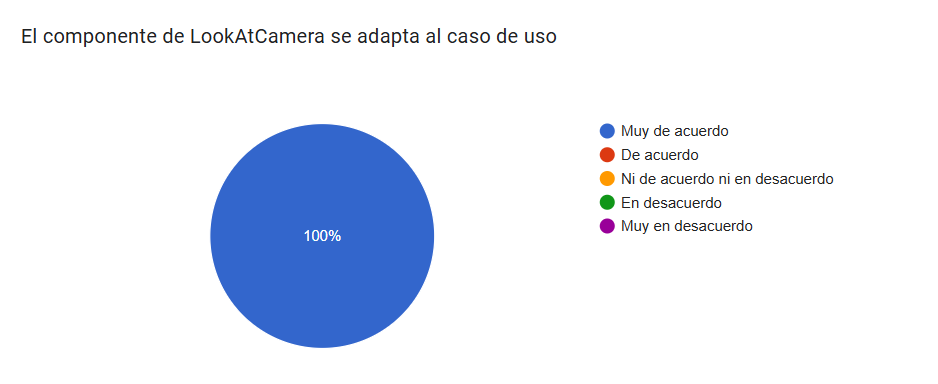
\includegraphics[width=450px,clip=true]{CUESTIONARIO_25.png}
  \caption{Encuesta sobre la utilidad del componente LookAtCamera.}
  \label{fig:CUESTIONARIO_25}
\end{figure}
\raggedbottom

\begin{figure}[H]
  \centering
  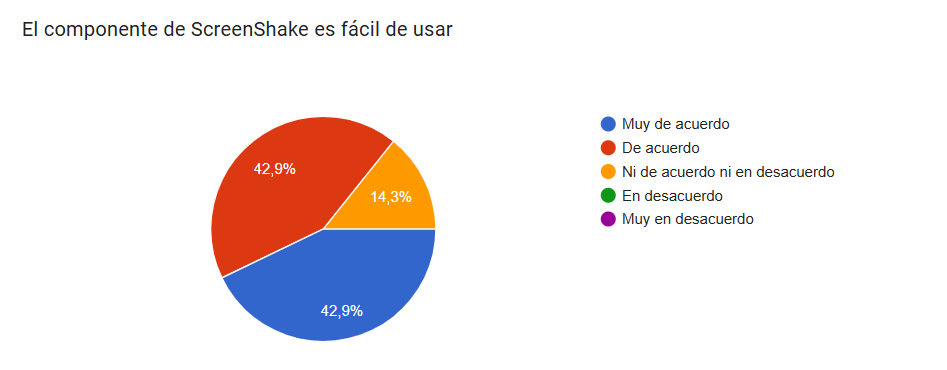
\includegraphics[width=450px,clip=true]{CUESTIONARIO_26.png}
  \caption{Encuesta sobre la facilidad de uso del componente de sacudida de cámara.}
  \label{fig:CUESTIONARIO_26}
\end{figure}
\raggedbottom

\begin{figure}[H]
  \centering
  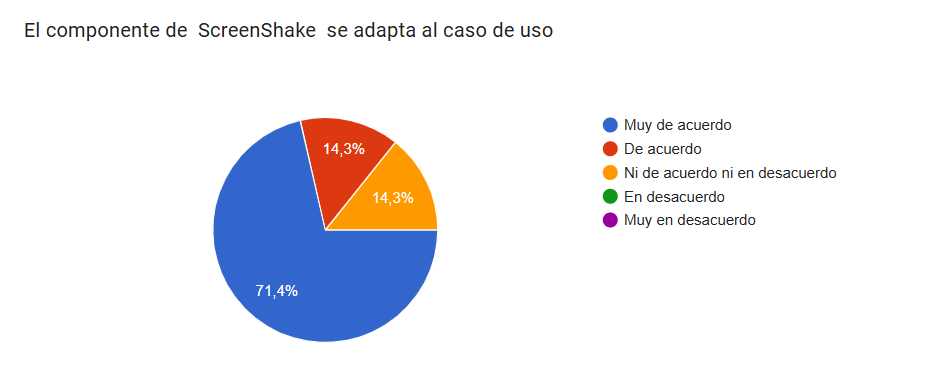
\includegraphics[width=450px,clip=true]{CUESTIONARIO_27.png}
  \caption{Encuesta sobre la utilidad del componente de sacudida de cámara.}
  \label{fig:CUESTIONARIO_27}
\end{figure}
\raggedbottom

\begin{figure}[H]
  \centering
  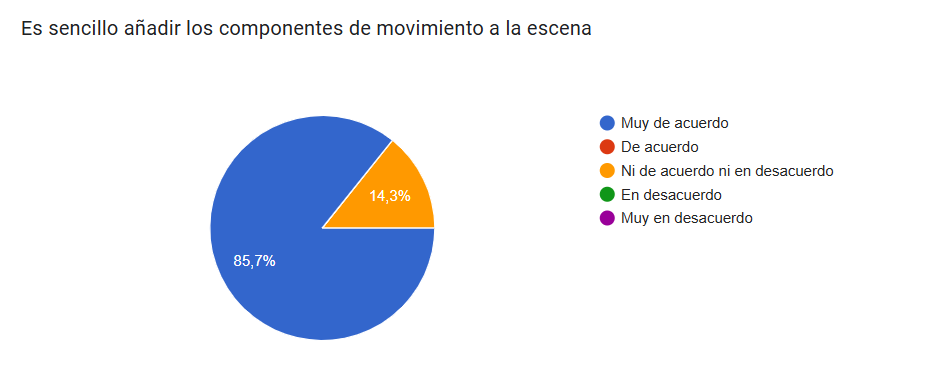
\includegraphics[width=450px,clip=true]{CUESTIONARIO_28.png}
  \caption{Encuesta sobre la facilidad de uso de los componentes de movimiento.}
  \label{fig:CUESTIONARIO_28}
\end{figure}
\raggedbottom

\begin{figure}[H]
  \centering
  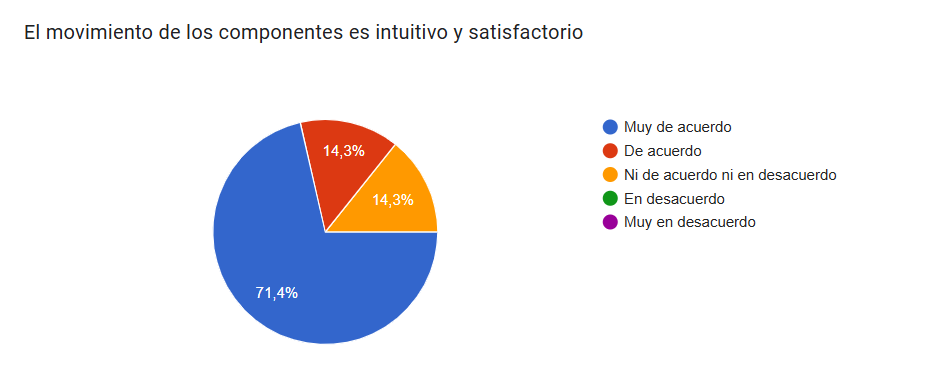
\includegraphics[width=450px,clip=true]{CUESTIONARIO_29.png}
  \caption{Encuesta sobre la efectividad de los componentes de movimiento.}
  \label{fig:CUESTIONARIO_29}
\end{figure}
\raggedbottom

\begin{figure}[H]
  \centering
  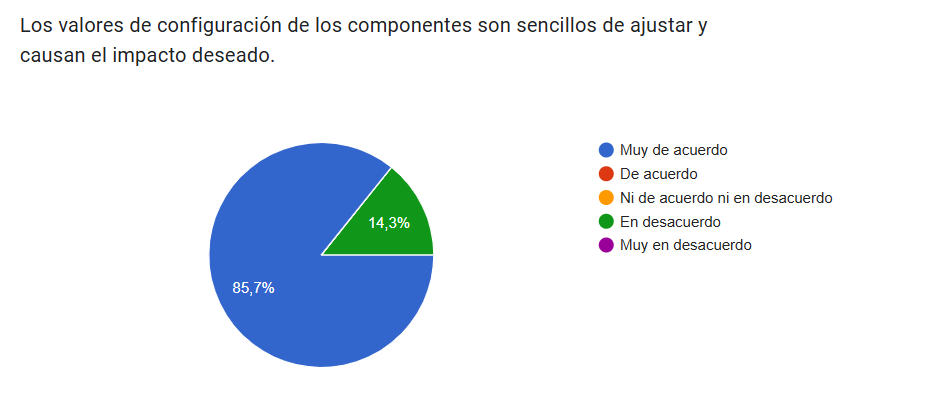
\includegraphics[width=450px,clip=true]{CUESTIONARIO_30.png}
  \caption{Encuesta sobre la facilidad de ajuste de los componentes de movimiento.}
  \label{fig:CUESTIONARIO_30}
\end{figure}
\raggedbottom

\begin{figure}[H]
  \centering
  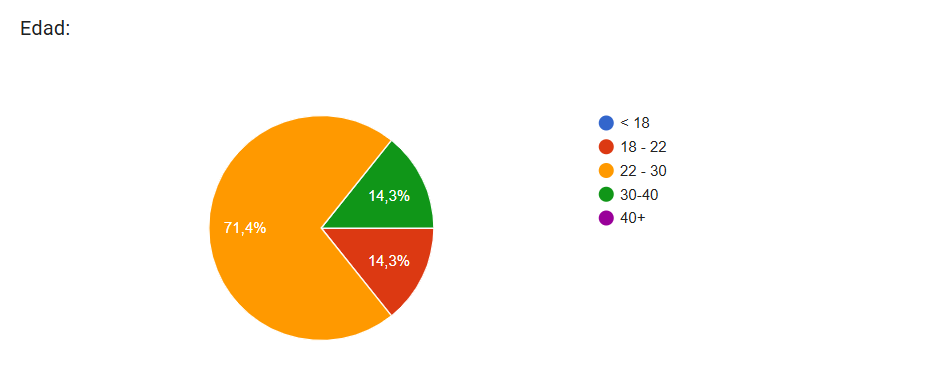
\includegraphics[width=450px,clip=true]{CUESTIONARIO_31.png}
  \caption{Encuesta sobre la edad del encuestado.}
  \label{fig:CUESTIONARIO_31}
\end{figure}
\raggedbottom

\begin{figure}[H]
  \centering
  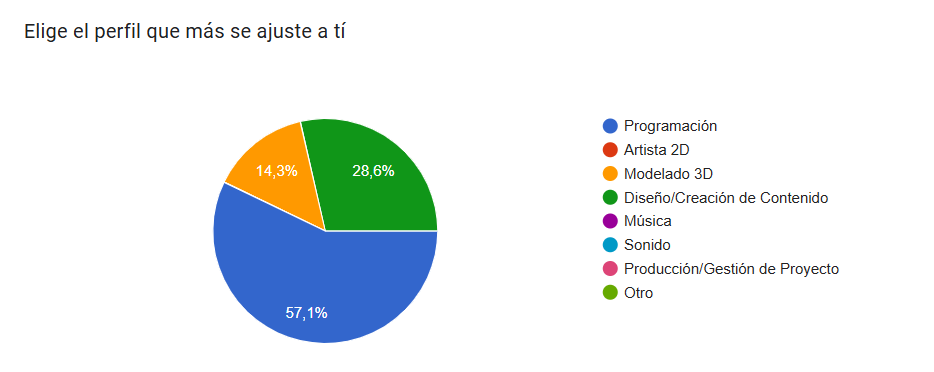
\includegraphics[width=450px,clip=true]{CUESTIONARIO_32.png}
  \caption{Encuesta sobre el perfil del encuestado.}
  \label{fig:CUESTIONARIO_32}
\end{figure}
\raggedbottom

\begin{figure}[H]
  \centering
  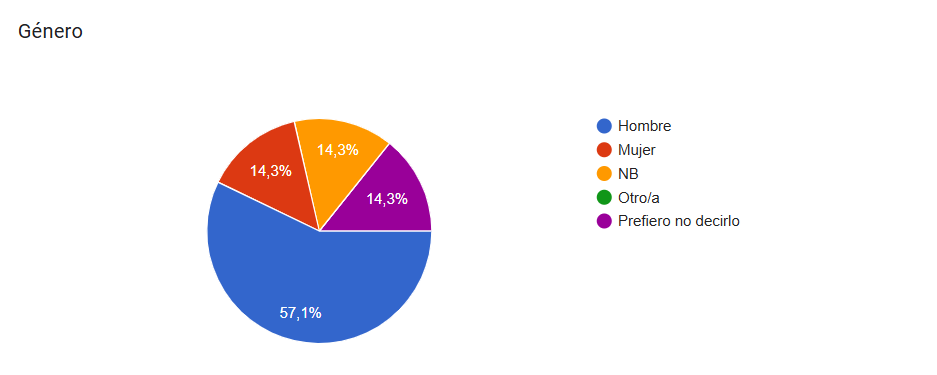
\includegraphics[width=450px,clip=true]{CUESTIONARIO_33.png}
  \caption{Encuesta sobre el género del encuestado.}
  \label{fig:CUESTIONARIO_33}
\end{figure}
\raggedbottom


\begin{table}[H]
  \begin{center}
  \setlength{\tabcolsep}{5pt}
  \renewcommand{\arraystretch}{1.2}
  \begin{tabular}{ | m{\textwidth} | } 
    \hline
    'Algunas de las funcionalidades de la librería están muy orientadas a programadores, cosas como ampliar las animaciones de texto no son viables para alguien sin (o con pocos) conocimientos técnicos. En cuanto a las funcionalidades que no 
    requieren programar, la librería resulta muy útil y dinámica para prototipar.' \\ 

    'Es sorprendente lo cómodo que se hace utilizar el sistema de diálogo. Por lo que he visto, el código está muy bien comentado y es, por lo general, fácil de leer.' \\ 

    'El componente SnapToGrid sería más útil si se pudiese utilizar en gameplay.' \\ 

    'Gran librería, la documentación sería un poco mejorable pero muy buen trabajo!' \\ 

    'El generador de mazmorras resulta ligeramente complejo de usar sin un trasfondo técnico, lo demás está muy guay' \\ 
    \hline
  \end{tabular}
  \centering
  \caption{¿Algún feedback adicional que quieras comentar?}
  \label{fig:tablaFeedback}
  \end{center}
\end{table}  


% También con \pagebreak